\documentclass[12pt,a4paper]{article}
\usepackage[utf8]{vietnam}
\usepackage{amsmath,amssymb}
\usepackage{tabularx}
\usepackage{tikz}
\usetikzlibrary{calc,angles,quotes,arrows.meta,patterns}
\usepackage{xcolor}
\usepackage{enumitem}
\usepackage{fancyhdr}
\usepackage[top=1.2cm, bottom=1.2cm, left=1.5cm, right=1.5cm]{geometry}
\usepackage[loigiai]{ex_test}
\SAOPTN{widthSA=2.6,heightSA=0.62}

\setlength{\headheight}{15pt}
\setlength{\parskip}{0pt}

\pagestyle{fancy}
\fancyhf{}
\rhead{\textit{Môn Toán 6 -- Hướng dẫn giải Đề số 8}}
\lhead{\textit{Bộ đề ôn tập Giữa học kì I}}
\cfoot{\thepage}

\begin{document}

\begin{center}
  \textbf{\Large HƯỚNG DẪN GIẢI CHI TIẾT VÀ BẢNG ĐÁP ÁN}\\
  \textbf{\large ĐỀ ÔN TẬP GIỮA HỌC KỲ I -- ĐỀ SỐ 8}\\
  \textit{Môn: Toán 6 -- Năm học 2026 -- 2027}
\end{center}
\vspace{2mm}

% --- BẢNG ĐÁP ÁN TRẮC NGHIỆM TÓM TẮT ---
\noindent\textbf{\large A. BẢNG ĐÁP ÁN TRẮC NGHIỆM TỔNG HỢP}
\vspace{1.5mm}

\noindent\textbf{1. Phần I (Mỗi câu trả lời đúng được 0,25 điểm):}
\begin{center}
\begin{tabular}{|c|c|c|c|c|c|c|c|c|c|c|c|c|}
\hline
\textbf{Câu} & \textbf{1} & \textbf{2} & \textbf{3} & \textbf{4} & \textbf{5} & \textbf{6} & \textbf{7} & \textbf{8} & \textbf{9} & \textbf{10} & \textbf{11} & \textbf{12} \\
\hline
\textbf{Đ/A} & \textbf{C} & \textbf{C} & \textbf{D} & \textbf{B} & \textbf{B} & \textbf{A} & \textbf{D} & \textbf{B} & \textbf{A} & \textbf{C} & \textbf{C} & \textbf{A} \\
\hline
\end{tabular}
\end{center}
\vspace{1mm}

\noindent\textbf{2. Phần II (Đúng 1 ý: 0,1đ; 2 ý: 0,25đ; 3 ý: 0,5đ; 4 ý: 1,0đ):}
\begin{center}
\begin{tabular}{|c|c|c|c|c||c|c|c|c|c|}
\hline
\textbf{Câu} & \textbf{a)} & \textbf{b)} & \textbf{c)} & \textbf{d)} & \textbf{Câu} & \textbf{a)} & \textbf{b)} & \textbf{c)} & \textbf{d)} \\
\hline
\textbf{Câu 1} & \textbf{Đ} & \textbf{Đ} & \textbf{Đ} & \textbf{S} & \textbf{Câu 2} & \textbf{Đ} & \textbf{S} & \textbf{Đ} & \textbf{Đ} \\
\hline
\end{tabular}
\end{center}
\vspace{1mm}

\noindent\textbf{3. Phần III (Mỗi câu trả lời đúng được 1,0 điểm):}
\begin{center}
\begin{tabular}{|c|c|c|}
\hline
\textbf{Câu} & \textbf{Câu 1} & \textbf{Câu 2} \\
\hline
\textbf{Đáp án} & \textbf{2} & \textbf{10} \\
\hline
\end{tabular}
\end{center}
\vspace{3mm}

% --- B. LỜI GIẢI CHI TIẾT ---
\noindent\textbf{\large B. LỜI GIẢI CHI TIẾT CÁC CÂU HỎI}
\vspace{2mm}

\noindent\textbf{\large PHẦN I. CÂU TRẮC NGHIỆM NHIỀU PHƯƠNG ÁN LỰA CHỌN}
\vspace{1mm}
\begin{ex}
Trong các số $23\,755; 10\,230; 17\,280; 18\,711$, số nào chia hết cho cả $2; 3; 5; 9$?
\choice
{$23\,755$}
{$10\,230$}
{\True $17\,280$}
{$18\,711$}
\loigiai{
Số chia hết cho cả 2 và 5 có chữ số tận cùng là 0, do đó chỉ xét $10\,230$ và $17\,280$.\\Xét tổng các chữ số:\\-- Số $10\,230$ có tổng chữ số là $1 + 0 + 2 + 3 + 0 = 6$ (không chia hết cho 9).\\-- Số $17\,280$ có tổng chữ số là $1 + 7 + 2 + 8 + 0 = 18$ (chia hết cho 9).\\Vậy số chia hết cho cả $2; 3; 5; 9$ là $17\,280$.
}
\end{ex}

\begin{ex}
Cho $A = \{x \in \mathbb{N}^* \mid x \le 12\}$. Tập hợp $A$ có số phần tử là:
\choice
{$10$}
{$11$}
{\True $12$}
{$13$}
\loigiai{
Các số tự nhiên khác 0 nhỏ hơn hoặc bằng 12 là $A = \{1; 2; 3; \dots; 12\}$. Tập hợp $A$ có 12 phần tử.
}
\end{ex}

\begin{ex}
Cho $18 \ \vdots \ x$ và $7 \le x < 18$. Khi đó $x$ có giá trị là:
\choice
{$2$}
{$3$}
{$6$}
{\True $9$}
\loigiai{
Các ước của 18 là $\{1; 2; 3; 6; 9; 18\}$. Giá trị thỏa mãn $7 \le x < 18$ là $x = 9$.
}
\end{ex}

\begin{ex}
Số nào sau đây không phải số nguyên tố?
\choice
{$11$}
{\True $33$}
{$17$}
{$31$}
\loigiai{
Số $33$ chia hết cho 3 và 11 nên là hợp số.
}
\end{ex}

\begin{ex}
Phân tích số $40$ ra thừa số nguyên tố ta được kết quả đúng là:
\choice
{$2 \cdot 4 \cdot 5$}
{\True $2^3 \cdot 5$}
{$5 \cdot 8$}
{$4 \cdot 10$}
\loigiai{
Ta có: $40 = 8 \cdot 5 = 2^3 \cdot 5$.
}
\end{ex}

\begin{ex}
Cho hình lục giác đều $ABCDEG$ tâm $O$. Khẳng định nào sau đây là đúng?
\begin{center}
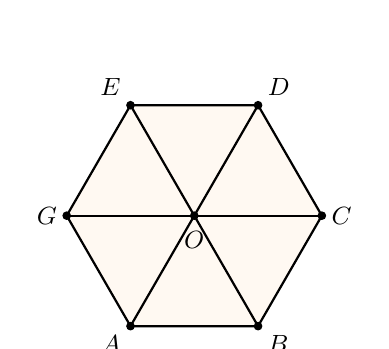
\begin{tikzpicture}[scale=0.9, font=\small]
  \coordinate (O) at (0,0);
  \foreach \i/\name in {0/C, 60/D, 120/E, 180/G, 240/A, 300/B} {
    \coordinate (\name) at (\i:1.8);
  }
  \draw[thick, fill=orange!5] (A) -- (B) -- (C) -- (D) -- (E) -- (G) -- cycle;
  \draw[thick] (A) -- (D);
  \draw[thick] (B) -- (E);
  \draw[thick] (C) -- (G);
  \filldraw (O) circle (1.5pt) node[below=2pt] {$O$};
  \filldraw (A) circle (1.5pt) node[below left] {$A$};
  \filldraw (B) circle (1.5pt) node[below right] {$B$};
  \filldraw (C) circle (1.5pt) node[right] {$C$};
  \filldraw (D) circle (1.5pt) node[above right] {$D$};
  \filldraw (E) circle (1.5pt) node[above left] {$E$};
  \filldraw (G) circle (1.5pt) node[left] {$G$};
\end{tikzpicture}
\end{center}
\choice
{\True $OA = OB = OC = OD = OE = OG$}
{$OA < OB < OC < OD < OE < OG$}
{$OA > OB > OC > OD > OE > OG$}
{$OA \ne OB \ne OC \ne OD \ne OE \ne OG$}
\loigiai{
Trong lục giác đều, khoảng cách từ tâm $O$ đến các đỉnh đều bằng nhau: $OA = OB = OC = OD = OE = OG$.
}
\end{ex}

\begin{ex}
Khẳng định nào sau đây là sai?
\choice
{Hình chữ nhật và hình thoi có các cặp cạnh đối song song với nhau}
{Hình lục giác đều có ba đường chéo chính bằng nhau}
{Hình bình hành có các cạnh đối bằng nhau}
{\True Hình thoi có hai đường chéo bằng nhau}
\loigiai{
Hai đường chéo của hình thoi vuông góc với nhau tại trung điểm mỗi đường chứ nói chung không bằng nhau (chỉ bằng nhau khi hình thoi là hình vuông).
}
\end{ex}

\begin{ex}
Hình nào sau đây có tất cả các góc ở đỉnh bằng nhau?
\choice
{Hình thoi}
{\True Hình chữ nhật}
{Hình bình hành}
{Hình thang cân}
\loigiai{
Hình chữ nhật có bốn góc ở đỉnh bằng nhau và đều bằng $90^\circ$.
}
\end{ex}

\begin{ex}
Một hình thang cân có độ dài hai đáy là $a, b$ và chiều cao là $h$. Công thức tính diện tích hình thang đó là:
\choice
{\True $S = \dfrac{(a+b) \cdot h}{2}$}
{$S = \dfrac{(a-b) \cdot h}{2}$}
{$S = 2(a+b) \cdot h$}
{$S = \dfrac{a+b}{2} \cdot h^2$}
\loigiai{
Diện tích hình thang bằng tổng độ dài hai đáy nhân với chiều cao rồi chia cho 2: $S = \dfrac{(a+b) \cdot h}{2}$.
}
\end{ex}

\begin{ex}
Cho hình thoi $ABCD$, hai đường chéo $AC$ và $BD$ của hình thoi:
\choice
{Bằng nhau}
{Không vuông góc}
{\True Vuông góc với nhau}
{Cả A và B đều đúng}
\loigiai{
Hai đường chéo của hình thoi luôn vuông góc với nhau.
}
\end{ex}

\begin{ex}
Viết gọn tích $8 \cdot 8 \cdot 2 \cdot 4$ dưới dạng lũy thừa cơ số 8 là:
\choice
{$8$}
{$8^2$}
{\True $8^3$}
{$8^4$}
\loigiai{
Ta có $2 \cdot 4 = 8$, do đó: $8 \cdot 8 \cdot 2 \cdot 4 = 8 \cdot 8 \cdot 8 = 8^3$.
}
\end{ex}

\begin{ex}
Một mảnh vườn hình chữ nhật có chiều dài $5\text{ m}$, chiều rộng $3\text{ m}$. Bác Bình muốn rào kín xung quanh mảnh vườn. Hỏi chiều dài hàng rào cần dùng là bao nhiêu mét?
\begin{center}
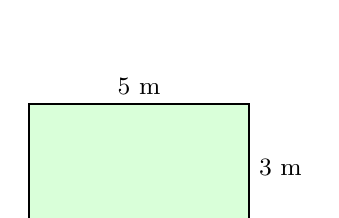
\begin{tikzpicture}[scale=0.8, font=\small]
  \coordinate (A) at (0,2);
  \coordinate (B) at (3.5,2);
  \coordinate (C) at (3.5,0);
  \coordinate (D) at (0,0);
  \draw[thick, fill=green!15] (A) -- (B) -- (C) -- (D) -- cycle;
  \node[above] at (1.75,2) {$5\text{ m}$};
  \node[right] at (3.5,1) {$3\text{ m}$};
\end{tikzpicture}
\end{center}
\choice
{\True $16\text{ m}$}
{$10\text{ m}$}
{$8\text{ m}$}
{$6\text{ m}$}
\loigiai{
Chiều dài hàng rào chính là chu vi của mảnh vườn hình chữ nhật:\\$\mathcal{P} = (5 + 3) \cdot 2 = 16\text{ (m)}$.
}
\end{ex}


\setcounter{ex}{0}
\vspace{2mm}
\noindent\textbf{\large PHẦN II. CÂU TRẮC NGHIỆM ĐÚNG SAI}
\vspace{1mm}
\begin{ex}
Cho các hình sau: tam giác đều, hình vuông, lục giác đều, hình chữ nhật, hình thoi, hình bình hành, hình thang cân. Xét tính đúng/sai của các khẳng định sau:
\choiceTF
{\True Hình tam giác đều, hình vuông, hình lục giác đều có tất cả các cạnh bằng nhau}
{\True Có đúng 2 hình có hai đường chéo vuông góc với nhau}
{\True Có đúng 3 hình có các cạnh đối song song và hai đường chéo bằng nhau}
{Hình lục giác đều có độ dài mọi đường chéo đều gấp đôi độ dài cạnh}
\loigiai{
\textbf{a)} Đúng. Tam giác đều, hình vuông và lục giác đều đều có đặc điểm là tất cả các cạnh bằng nhau.

\textbf{b)} Đúng. Hai hình có hai đường chéo vuông góc với nhau là hình vuông và hình thoi.

\textbf{c)} Đúng. Ba hình thỏa mãn điều kiện có hai cạnh đối song song và hai đường chéo bằng nhau là hình chữ nhật, hình vuông và hình thang cân.

\textbf{d)} Sai. Trong lục giác đều, chỉ có 3 đường chéo chính mới có độ dài gấp đôi cạnh, các đường chéo phụ không có tính chất này.
}
\end{ex}

\begin{ex}
Một chiếc ô tô đang di chuyển với vận tốc ban đầu là $10\text{ km/h}$. Sau mỗi giờ, vận tốc tăng gấp đôi. Xét tính đúng/sai của các khẳng định sau:
\choiceTF
{\True Sau 1 giờ, vận tốc ô tô là $20\text{ km/h}$}
{Sau 2 giờ, vận tốc ô tô là $30\text{ km/h}$}
{\True Sau 3 giờ, vận tốc ô tô là $80\text{ km/h}$}
{\True Sau 4 giờ, vận tốc ô tô là $160\text{ km/h}$}
\loigiai{
\textbf{a)} Đúng. Vận tốc ban đầu là $10\text{ km/h}$, sau 1 giờ đạt $10 \cdot 2 = 20\text{ km/h}$.

\textbf{b)} Sai. Sau 2 giờ, vận tốc tăng gấp đôi so với giờ thứ nhất, đạt $20 \cdot 2 = 40\text{ km/h}$.

\textbf{c)} Đúng. Sau 3 giờ, vận tốc đạt $40 \cdot 2 = 80\text{ km/h}$.

\textbf{d)} Đúng. Sau 4 giờ, vận tốc đạt $80 \cdot 2 = 160\text{ km/h}$.
}
\end{ex}


\setcounter{ex}{0}
\vspace{2mm}
\noindent\textbf{\large PHẦN III. CÂU HỎI TRẢ LỜI NGẮN}
\vspace{1mm}
\begin{ex}
Có bao nhiêu số tự nhiên $m$ sao cho $5 < m < 10$ và $m$ chia hết cho 3? \shortans{2}
\loigiai{
Các số tự nhiên $m$ thỏa mãn $5 < m < 10$ là $\{6; 7; 8; 9\}$.\\Trong các số trên, các số chia hết cho 3 là 6 và 9.\\Vậy có 2 số tự nhiên thỏa mãn đề bài.
}
\end{ex}

\begin{ex}
Một hình chữ nhật có diện tích là $120\text{ cm}^2$ và có chiều dài là $12\text{ cm}$. Tính độ dài chiều rộng của hình chữ nhật đó (theo đơn vị $\text{cm}$). \shortans{10}
\loigiai{
Độ dài chiều rộng của hình chữ nhật là: $120 : 12 = 10\text{ (cm)}$.
}
\end{ex}


\setcounter{ex}{0}
\vspace{2mm}
\noindent\textbf{\large PHẦN IV. TỰ LUẬN (BÀI TẬP VÀ BAREM ĐIỂM)}
\vspace{1mm}
\begin{ex} (1,0 điểm)
Thực hiện phép tính (Tính nhanh nếu có thể):
\begin{enumerate}[label=\textbf{\alph*)}, leftmargin=0.8cm, itemsep=2pt]
\item (0,5 điểm) $127 + 156 + 73 + 144$
\item (0,5 điểm) $2026 - (20 \cdot 3^2 + 16 : 2^2)$
\end{enumerate}
\loigiai{
\textbf{a)} \textbf{[0,5 điểm]}\\ $(127 + 73) + (156 + 144) = 200 + 300 = 500$.

\textbf{b)} \textbf{[0,5 điểm]}\\ $2026 - (20 \cdot 9 + 16 : 4) = 2026 - (180 + 4) = 2026 - 184 = 1842$.


}
\end{ex}
\vspace{2mm}

\begin{ex} (1,0 điểm)
Tìm số tự nhiên $x$, biết:
\begin{enumerate}[label=\textbf{\alph*)}, leftmargin=0.8cm, itemsep=2pt]
\item (0,5 điểm) $x - 18 = 15$
\item (0,5 điểm) $18 + 2(x - 1) = 40$
\end{enumerate}
\loigiai{
\textbf{a)} \textbf{[0,5 điểm]}\\ $x = 15 + 18 \Rightarrow x = 33$.

\textbf{b)} \textbf{[0,5 điểm]}\\ $2(x - 1) = 40 - 18 \Rightarrow 2(x - 1) = 22 \Rightarrow x - 1 = 11 \Rightarrow x = 12$.


}
\end{ex}
\vspace{2mm}

\begin{ex} (0,5 điểm)
Một hình chữ nhật có diện tích là $220\text{ cm}^2$ và có chiều dài là $22\text{ cm}$. Tính độ dài chiều rộng của hình chữ nhật (theo đơn vị $\text{cm}$).
\loigiai{
Chiều rộng của hình chữ nhật là:\\$220 : 22 = 10\text{ (cm)}$.
}
\end{ex}
\vspace{2mm}

\begin{ex} (0,5 điểm)
Không thực hiện tính tổng, chứng minh rằng biểu thức sau chia hết cho 21:\\$A = 1 + 4 + 4^2 + 4^3 + \dots + 4^{2021}$
\loigiai{
Tổng $A$ có $2021 - 0 + 1 = 2022$ số hạng. Vì 2022 chia hết cho 3 nên ta nhóm 3 số hạng liên tiếp vào một nhóm:
\begin{align*}
A &= (1 + 4 + 4^2) + (4^3 + 4^4 + 4^5) + \dots + (4^{2019} + 4^{2020} + 4^{2021})\\
&= (1 + 4 + 16) + 4^3 \cdot (1 + 4 + 16) + \dots + 4^{2019} \cdot (1 + 4 + 16)\\
&= 21 + 4^3 \cdot 21 + \dots + 4^{2019} \cdot 21\\
&= 21 \cdot (1 + 4^3 + \dots + 4^{2019})
\end{align*}
Vì tích có thừa số 21 nên $A \ \vdots \ 21$ (đpcm).
}
\end{ex}
\vspace{2mm}


\begin{center}
\rule{4cm}{0.4pt}\\
\textit{--- HẾT ---}
\end{center}
\end{document}
